\documentclass[aspectratio=169, 10pt]{beamer}

% === PREÁMBULO ===
\usepackage[utf8]{inputenc}
\usepackage[spanish]{babel}
\usepackage{graphicx}
\usepackage{amsmath}
\usepackage{amssymb}
\usepackage{tikz}
\usetikzlibrary{positioning}
\usepackage{booktabs}
\usepackage{tcolorbox}

% === PALETA DE COLORES ===
\definecolor{C1}{RGB}{20, 80, 60}       % verde oscuro — estructura
\definecolor{C2}{RGB}{46, 139, 104}     % verde medio — acento
\definecolor{C3}{RGB}{210, 240, 225}    % verde muy claro — fondo bloque
\definecolor{CA}{RGB}{180, 100, 20}     % naranja — alerta / énfasis
\definecolor{CG}{RGB}{245, 245, 242}    % gris cálido — fondo slide
\definecolor{CT}{RGB}{30, 30, 30}       % texto principal

% === TEMA Y COLORES ===
\usetheme{Madrid}
\usecolortheme{default}

% === CONFIGURAR COLORES BEAMER ===
\setbeamercolor{normal text}{fg=CT, bg=CG}
\setbeamercolor{frametitle}{fg=white, bg=C1}
\setbeamercolor{structure}{fg=C1}
\setbeamercolor{block title}{bg=C1, fg=white}
\setbeamercolor{block body}{bg=C3}
\setbeamercolor{block title alerted}{bg=CA, fg=white}
\setbeamercolor{block body alerted}{bg=CA!12}
\setbeamercolor{block title example}{bg=C2, fg=white}
\setbeamercolor{block body example}{bg=C2!15}
\setbeamertemplate{itemize item}{\color{C2}\textbullet}
\setbeamertemplate{itemize subitem}{\color{C2}$\circ$}

% === ELIMINAR BARRA DE NAVEGACIÓN ===
\setbeamertemplate{navigation symbols}{}

% === PIE DE PÁGINA: SOLO NÚMERO DE FILMINA ===
\setbeamertemplate{footline}{
  \hbox{%
    \begin{beamercolorbox}[wd=\paperwidth,ht=2.25ex,dp=1ex,right]{date in head/foot}%
      \usebeamerfont{date in head/foot}%
      \insertframenumber{} / \inserttotalframenumber\hspace*{2ex}
    \end{beamercolorbox}%
  }%
  \vskip0pt%
}

% === TAMAÑOS DE FUENTES ===
\setbeamerfont{frametitle}{size=\large, series=\bfseries}
\setbeamerfont{title}{size=\Large, series=\bfseries}
\setbeamerfont{block title}{series=\bfseries, size=\small}
\setbeamerfont{block body}{size=\small}
\setbeamerfont{itemize/enumerate body}{size=\normalsize}

% === INFORMACIÓN DEL DOCUMENTO ===
\title{Inteligencia Artificial para la Predicción
Automática de Parámetros Geométricos
en Moldes Nanoestructurados}
\subtitle{}
\author{Agustín Ottaviano \\ \small Director: Fernando Meneses}
\institute{Universidad Nacional de Córdoba}
\date{\today}

% === LOGO (OPCIONAL) ===
% \logo{\includegraphics[height=1.5cm]{logo.png}}

\begin{document}

% ============================================
% DIAPOSITIVA DE TÍTULO
% ============================================
\frame{\titlepage}

% ============================================
% TABLA DE CONTENIDOS
% ============================================
\begin{frame}{Contenido}
    \tableofcontents
\end{frame}

% ============================================
% CAPÍTULOS
% ============================================

% ============================================
% SECCIÓN 1: Motivación
% ============================================
\section{Motivación}

\begin{frame}{El problema: Medir la geometría de los poros}
    \begin{columns}[T]
        \column{0.5\textwidth}

        \begin{block}{Material: AAO}
            Membrana nanoestructurada con poros cilíndricos organizados en red hexagonal. Sus propiedades ópticas y mecánicas dependen de la geometría de los poros.
        \end{block}

        \begin{block}{Objetivo}
            Predecir automáticamente los parámetros geométricos de una imagen SEM.
        \end{block}

        \begin{alertblock}{5 variables objetivo}
            \renewcommand{\arraystretch}{1.25}
            \begin{tabular}{@{}ll@{}}
              $R$,\;$\sigma_R$       & Radio promedio y dispersión [px] \\
              $DCC$,\;$\sigma_{DCC}$ & Distancia centro a centro [px] \\
              $P$                    & Porosidad (\%) \\
            \end{tabular}
        \end{alertblock}

        \column{0.5\textwidth}

        \begin{center}
            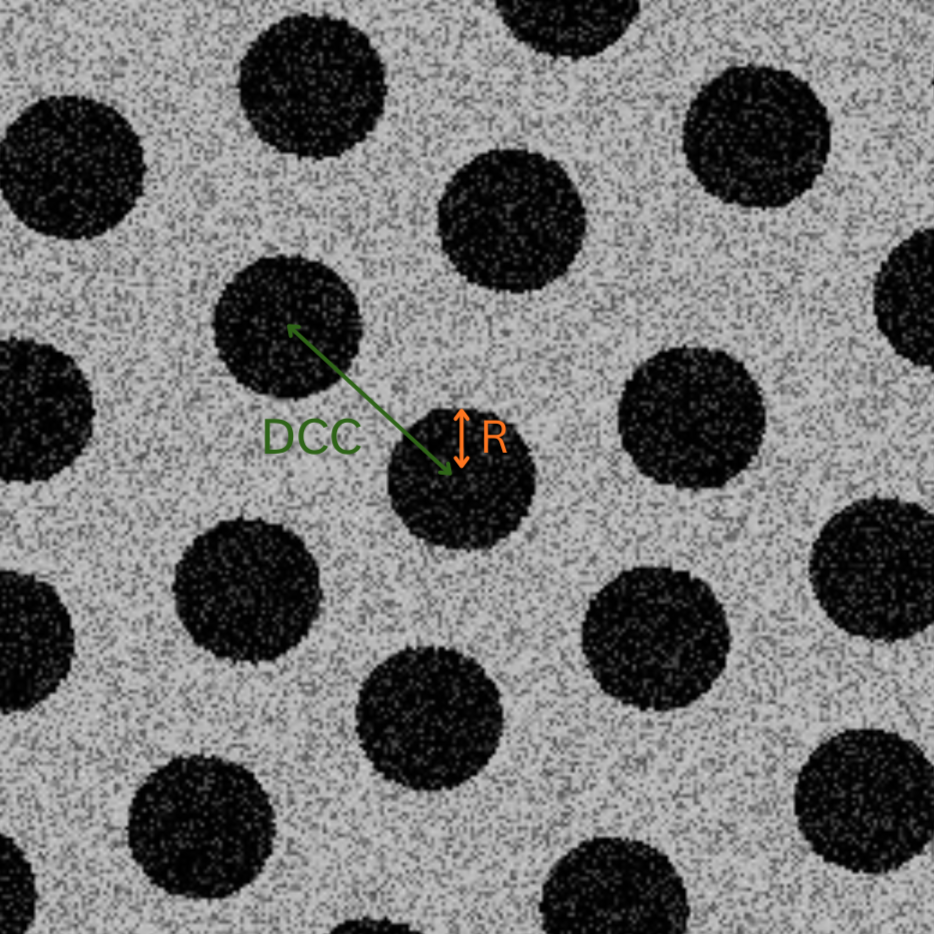
\includegraphics[width=0.7\textwidth]{chapters/introduction/ImagenAAO.png}
        \end{center}

    \end{columns}
\end{frame}


% ============================================
% SECCIÓN 2: Generación del Dataset Simulado
% ============================================
\section{Generación del Dataset Simulado}

\begin{frame}{Generación del Dataset Simulado}

\begin{columns}[t]

% ---- COLUMNA IZQUIERDA (imágenes) ----
\column{0.25\textwidth}

    \begin{center}
        \begin{tcolorbox}[
        colback=C3,
        colframe=C2,
        boxrule=1pt,
        arc=6pt,
        width=1.4\textwidth,
        left=6pt, right=6pt,
        top=4pt, bottom=4pt,
        boxsep=2pt,
        center
        ]
        \small
        Se generaron \textbf{20\,000 imágenes} de $300\times300$ px. Cada imagen genera una fila en el CSV con variables: 
        $R$, $\sigma_R$, $DCC$, $\sigma_{DCC}$, $P$.
        \end{tcolorbox}        
    \end{center}

    \centering

    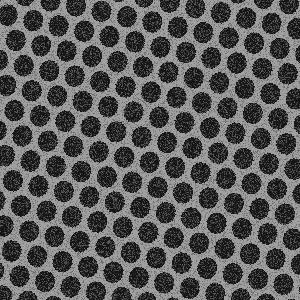
\includegraphics[width=0.45\textwidth]{chapters/metodologia/generada1.jpg}
    
\includegraphics[width=0.45\textwidth]{chapters/metodologia/generada2.jpg}

    \vspace{0.3cm}

    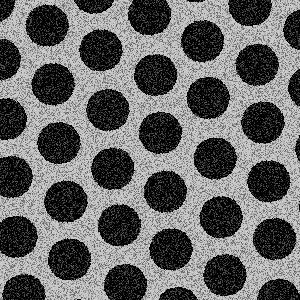
\includegraphics[width=0.45\textwidth]{chapters/metodologia/generada3.jpg}
    
\includegraphics[width=0.45\textwidth]{chapters/metodologia/generada4.jpg}    
    \column{0.60\textwidth}

% ---- COLUMNA DERECHA (tabla) ----

    \begin{block}{Parámetros aleatorios por imagen}
        \small
        \begin{itemize}
            \item \textbf{Radio} $r \in [10,30]$ px: tamaño promedio de los poros en la imagen simulada.
            \item \textbf{Distancia centro a centro} $dcc \in [2.5r,\,4.5r]$: garantiza que no se solapen y cubre distintas densidades de poros.
            \item \textbf{Desorden} en $r$ y $dcc$ (hasta $10\%$).
            \item \textbf{Rotación} $\theta \in [0^\circ,360^\circ]$.
            \item \textbf{Brillo} $B \in [-40,40]$: suma una constante a cada píxel, aclarando u oscureciendo la imagen.
            \item \textbf{Contraste} $C \in [0.6,1.4]$: escala el rango de grises; $C<1$ reduce la diferencia entre poros y fondo, $C>1$ la aumenta.
            \item \textbf{Ruido}: perturbación aleatoria pixel a pixel que simula el ruido electrónico del detector del microscopio.
        \end{itemize}
    \end{block} 

\end{columns}

\end{frame}

% ============================================
% SECCIÓN 3: Normalización de las labels
% ============================================
\section{Normalización de las labels}

\begin{frame}{Normalización de las Labels}
    \begin{columns}[T]
        \column{0.4\textwidth}
        
        \begin{block}{Por qué normalizar}
            Las variables tienen escalas muy distintas: $R \sim 20$ \, px pero  $P \sim 0.3$. Sin normalizar, las variables grandes dominan el MAE y el modelo aprende mal.
        \end{block}

        \begin{exampleblock}{StandardScaler}
            Técnica que transforma las variables:
            $$x_{\text{norm}} = \frac{x - \mu}{\sigma}$$
            donde $\mu$ y $\sigma$ son la media y la desviación estándar de cada variable, respectivamente.
            
            \textbf{Resultado:} media 0 y desv. est. 1.
        \end{exampleblock}
        
        \column{0.45\textwidth}
        
        \begin{exampleblock}{Transformación Inversa}
            Despejar $x$ de la ecuación:
            $$x = x_{norm} \cdot \sigma + \mu$$
            
            \textbf{Importante:} Los valores de $\mu$ y $\sigma$ se guardan.
        \end{exampleblock}
        
        \begin{block}{Flujo del proceso}
            \small
            \begin{enumerate}
                \item CSV Original con 5 variables
                \item Aplicar StandardScaler
                \item Guardar scaler
                \item Labels listas para entrenar
                \item Entrenar la red neuronal
                \item Evaluar la red neuronal y usar Scaler Inverso para obtener MAPE
            \end{enumerate}
        \end{block}
    \end{columns}
\end{frame}

% ============================================
% SECCIÓN 4: PIPELINE DE ENTRENAMIENTO
% ============================================
\section{Pipeline de Entrenamiento}

\begin{frame}{Transformación de Imágenes}
    \begin{block}{Valores originales}
        Las imágenes SEM vienen con píxeles en rango $[0, 255]$.
    \end{block}
    
    \begin{exampleblock}{Normalización de píxeles}
        Se transforman a uno de estos rangos:
        \begin{itemize}
            \item Rango $[0, 1]$: dividir por 255
            \item Rango $[-1, 1]$: dividir por 127.5 y restar 1
            \item Mantener $[0, 255]$: sin transformación
        \end{itemize}
    \end{exampleblock}
    
    \begin{alertblock}{¿Por qué?}
        Facilita la convergencia del modelo. Además, algunas arquitecturas de Transfer Learning (como VGG o ResNet) fueron entrenadas con imágenes en $[-1,1]$ o $[0,1]$, por lo que requieren esa misma normalización para funcionar correctamente.
    \end{alertblock}
\end{frame}

\begin{frame}{División del Dataset}

    \begin{block}{Partición de las 20\,000 imágenes}
        \small
        \begin{itemize}
            \item \textbf{Train Set} ($40\% \approx 8\,000$): el modelo ajusta sus pesos sobre este conjunto en cada época de entrenamiento.
            \item \textbf{Validation Set} ($20\% \approx 4\,000$): se evalúa al final de cada época para monitorear el aprendizaje sin usarlo para ajustar pesos.
            \item \textbf{Test Set} ($40\% \approx 8\,000$): se usa una única vez al final para reportar el desempeño real del modelo.
        \end{itemize}
    \end{block}

    \begin{center}
    \begin{tikzpicture}[font=\small]
        \fill[C1]  (0,0)    rectangle (4.80, 0.6);
        \fill[C2]  (4.80,0) rectangle (6.00, 0.6);
        \fill[CA]  (6.00,0) rectangle (10.0, 0.6);
        \draw[gray!60] (0,0) rectangle (10.0, 0.6);
        \node[white, font=\small\bfseries]      at (2.40, 0.30) {Train $40\%$};
        \node[white, font=\scriptsize\bfseries] at (5.40, 0.30) {Val $20\%$};
        \node[white, font=\small\bfseries]      at (8.00, 0.30) {Test $40\%$};
        \node[font=\scriptsize, text=C1] at (2.40, -0.30) {$\approx\!8\,000$ imágenes};
        \node[font=\scriptsize, text=C2] at (5.40, -0.30) {$\approx\!4\,000$};
        \node[font=\scriptsize, text=CA] at (8.00, -0.30) {$\approx\!8\,000$ imágenes};
    \end{tikzpicture}
    \end{center}

    \begin{block}{Entrenamiento}
        \small
        \begin{itemize}
            \item \textbf{Batch size} 32: en vez de actualizar los pesos de la red con una imagen a la vez, se acumulan 32 imágenes y se actualiza una sola vez. Reduce el ruido del aprendizaje y acelera el entrenamiento.
            \item \textbf{Épocas}: máximo 150, pero con early stopping: si la pérdida en Validation Set no mejora durante 20 épocas consecutivas, el entrenamiento se detiene antes para evitar sobreajuste y ahorrar tiempo.
        \end{itemize}
    \end{block}

\end{frame}

\begin{frame}{Entrenamiento del Modelo}
    \begin{block}{Arquitectura}
        Dos opciones:
        \begin{itemize}
            \item \textbf{CNN Completa}: Arquitectura de una red convolucional entrenada desde cero.
            \item \textbf{Transfer Learning}: Se utilizan capas de un modelo preentrenado y se le agregan capas convolucionales al final que son entrenadas acordes a lo que se necesita predecir. 
        \end{itemize}
    \end{block}
    
    \begin{block}{Datos de entrada}
        \begin{itemize}
            \item Imágenes: transformadas a $[0,1]$, $[-1,1]$ o $[0,255]$
            \item Labels: normalizados con StandardScaler
        \end{itemize}
    \end{block}
    
\end{frame}

\begin{frame}{Obtención del MAPE en Test Set}
    \begin{block}{Paso 1: Predicciones}
        El modelo entrenado realiza predicciones en Test Set:
        $$ \text{Modelo}(x_{\text{img}}) = \bigl(\hat{R}_{\text{norm}},\; \hat{\sigma}_{R,\text{norm}},\; \hat{DCC}_{\text{norm}},\; \hat{\sigma}_{DCC,\text{norm}},\; \hat{P}_{\text{norm}}\bigr) $$
    \end{block}
    
    \begin{block}{Paso 2: Scaler Inverso}
        Desnormalizamos las predicciones normalizadas aplicando la transformación inversa:
        $$(\hat{R},\; \hat{\sigma}_R,\; \hat{DCC},\; \hat{\sigma}_{DCC},\; \hat{P}) = \text{scaler.inverse\_transform}(\hat{R}_{\text{norm}},\; \hat{\sigma}_{R,\text{norm}},\; \ldots)$$
    \end{block}
    
    \begin{exampleblock}{Paso 3: Calcular MAPE}
        Calculamos MAPE para cada una de las variables en el Test Set:
        $$\text{MAPE} = \frac{1}{n}\sum_{i=1}^{n}\left|\frac{y_i - \hat{y}_i}{y_i}\right| \times 100\text{\%}$$
        donde $y_i$ son los labels reales del Test Set y $\hat{y}_i$ las predicciones.
    \end{exampleblock}
\end{frame}


% ============================================
% Evaluación en Dataset Externo Real
% ============================================
\section{Resultados}

% --- Slide 1: Presentación del dataset externo ---
\begin{frame}{Evaluación en Dataset Externo Real}
    \begin{columns}[T]
        \column{0.5\textwidth}

        \begin{block}{Dataset externo}
            Se utilizaron \textbf{24 imágenes SEM reales} (no simuladas) con sus parámetros geométricos medidos manualmente para evaluar la generalización del modelo.
        \end{block}

        \begin{alertblock}{Objetivo}
            Verificar si el modelo entrenado con imágenes simuladas es capaz de predecir correctamente los parámetros de imágenes reales.
        \end{alertblock}

        \begin{exampleblock}{Métrica}
            MAPE sobre $R$, $DCC$ y $P$ en espacio real (unidades originales).
        \end{exampleblock}

        \column{0.5\textwidth}

        \begin{center}
            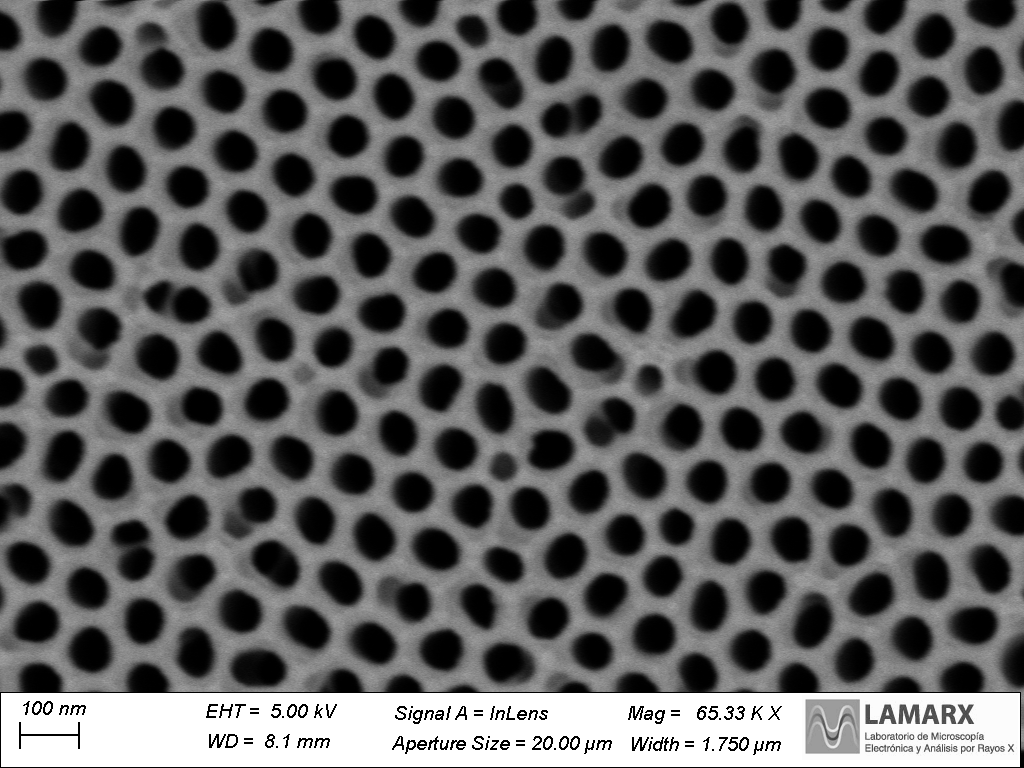
\includegraphics[width=0.9\textwidth]{chapters/Resultados/ImagenSEM.png}

            \small Imagen SEM real con franja de parámetros
        \end{center}

    \end{columns}
\end{frame}

% --- Slide 2: Desafíos, solución y pipeline ---
\begin{frame}{Evaluación en Dataset Externo Real: Pipeline}
    \begin{columns}[T]
        \column{0.5\textwidth}

        \begin{alertblock}{Desafíos de las imágenes SEM reales}
            \begin{enumerate}
                \item Las imágenes tienen resolución mas grande a la utilizada en el entrenamiento.
                \item Las imágenes suelen incluir una franja impresa con parámetros del microscopio (escala, voltaje, etc.).
            \end{enumerate}
        \end{alertblock}

        \begin{block}{Solución: recorte por esquina}
            Para cada imagen se seleccionó una esquina de $300\times300$ px libre de la franja de parámetros del microscopio.
        \end{block}

        \column{0.45\textwidth}

        \begin{exampleblock}{Pipeline de evaluación}
            \small
            \begin{enumerate}
                \item Leer labels en espacio real (sin estandarizar)
                \item Recortar cada imagen a $300\times300$ px sin franja de parámetros
                \item Normalizar píxeles igual que en el entrenamiento
                \item Obtener predicciones y convertirlas al espacio real
                \item Calcular MAPE sobre $R$, $DCC$, $P$
            \end{enumerate}
        \end{exampleblock}

    \end{columns}

    \begin{block}{Nota}
        Los parámetros reales de las imágenes SEM están en unidades originales. Las predicciones del modelo se desnormalizan antes de comparar, para que ambos estén en el mismo espacio.
    \end{block}

\end{frame}

% --- Slide 3: Resultados numéricos ---
\begin{frame}{Evaluación en Dataset Externo Real: Resultados}

    \begin{columns}[T]
        \column{0.30\textwidth}
        \begin{exampleblock}{MAPE — 24 imágenes SEM}
            \renewcommand{\arraystretch}{0.9}
            \begin{tabular}{@{}lc@{}}
            \toprule
            Variable & MAPE \\
            \midrule
            Radio $R$       & $11.00\%$ \\
            Distancia $DCC$ & $11.53\%$ \\
            Porosidad $P$   & $20.51\%$ \\
            \bottomrule
            \end{tabular}
        \end{exampleblock}

        \column{0.6\textwidth}
        \begin{block}{Conclusión}
            El modelo es aceptable: la mayoría de las imágenes presentan errores por debajo del $20\%$.
        \end{block}
    \end{columns}

    \vspace{0.1cm}
    \begin{center}
        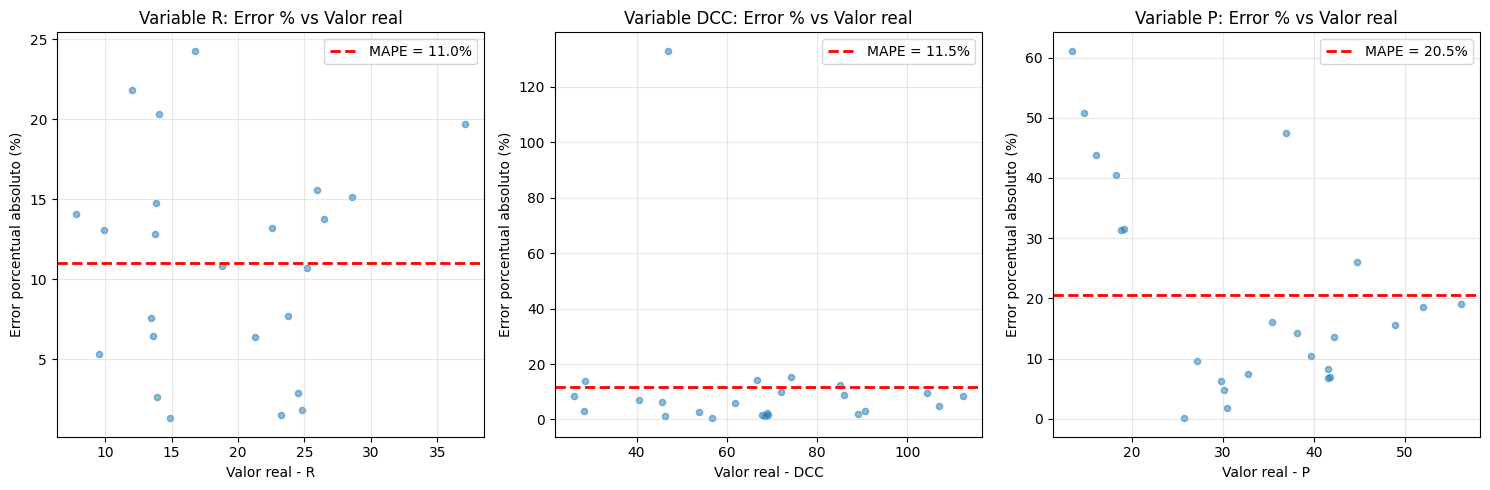
\includegraphics[width=0.8\textwidth]{chapters/Resultados/resultados_conv.png}
    \end{center}

\end{frame}

% ============================================
% DIAPOSITIVA FINAL
% ============================================

\begin{frame}[plain]
    \begin{center}
        {\Large \textbf{¡Gracias!}}
        
    \end{center}
\end{frame}


\end{document}
